\documentclass[12pt]{article}
\usepackage[latin1]{inputenc}
\usepackage{amsmath}
\usepackage{mathtools}
\usepackage{xspace}
\usepackage{graphicx}
\usepackage[english]{babel}
\usepackage[font=small,labelfont=bf]{caption}
\usepackage[centering,includeheadfoot,margin=2cm]{geometry}
\usepackage{tikz}
\usetikzlibrary{shapes,arrows,automata,trees, shadows,decorations.pathmorphing}
\title{CS375 WK5}
\author{Jason N Mansfield}
\begin{document}

\begin{figure}
\begin{center}
\caption{Q01: $L_1$ = (a+b)*a}
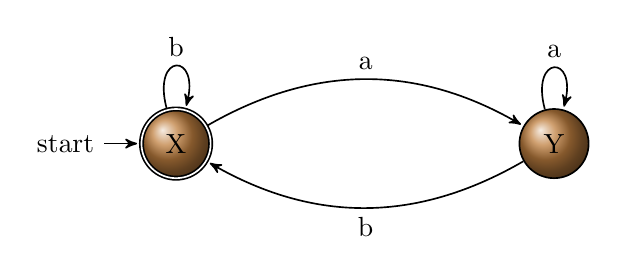
\begin{tikzpicture}[->,>=stealth',shorten >=1pt,auto,node distance=4.8cm, semithick]
\tikzstyle{every state}=[draw=black,text=black, ball color=brown]
\node[initial,state,accepting] (X) {X};
\node[state][right of=X](Y){Y};
\path (Y)edge [bend left] node{b}(X)
         edge  [loop above]node{a}(Y)
         (X)edge [loop above]node{b}(X)
         edge [bend left] node{a}(Y);
\end{tikzpicture} 
\end{center}
\end{figure}

\begin{figure}
\begin{center}
\caption{Q01: $L_2$= b(a+b)*}
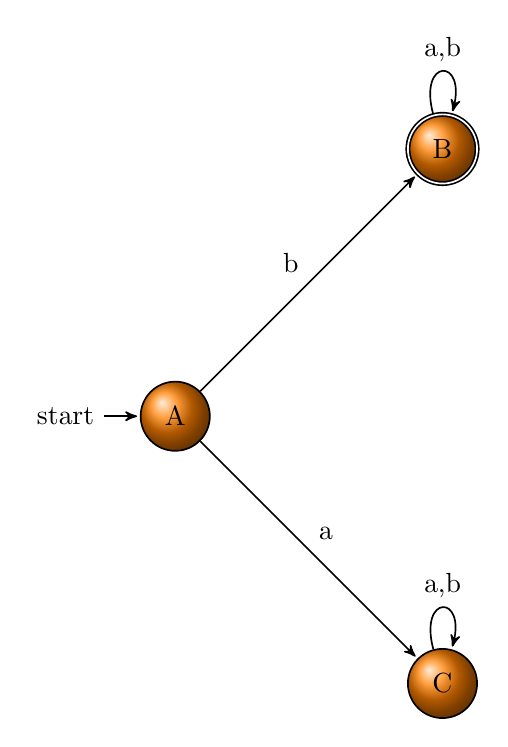
\begin{tikzpicture}[->,>=stealth',shorten >=1pt,auto,node distance=4.8cm, semithick]
\tikzstyle{every state}=[draw=black,text=black, ball color=orange]
\node[initial,state] (A) {A};
\node[state,accepting][above right of=A](B){B};
\node[state][below right of=A](C){C};
\path (A)edge node{b}(B)
         edge  node{a}(C)
      (B)edge  [loop above]node{a,b}(B)
      (C)edge [loop above]node{a,b}(C);
\end{tikzpicture} 
\end{center}
\end{figure}


\begin{figure}
\begin{center}
\caption{Q01: $L_1$$\bigcap$$L_2$}
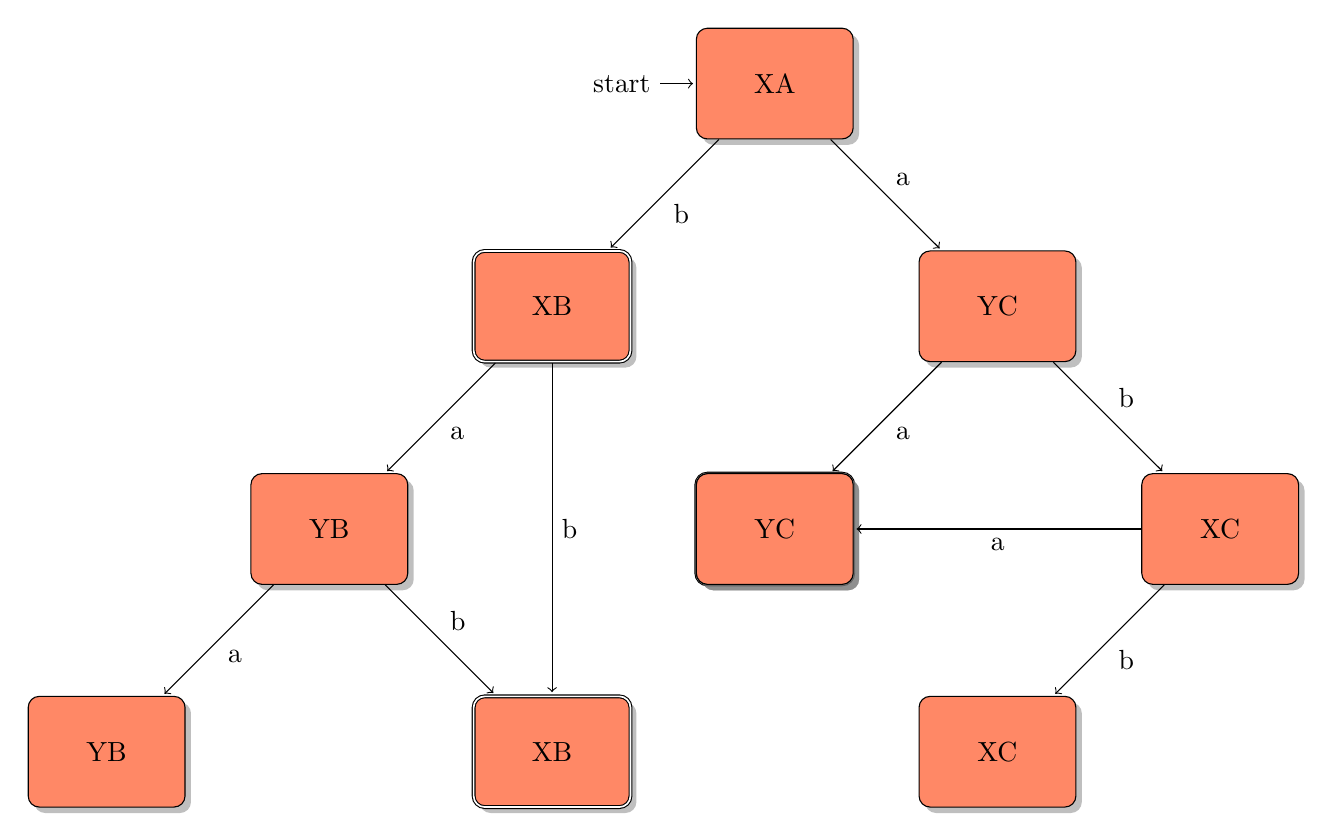
\begin{tikzpicture}[->,shorten >=1pt,node distance=4cm,auto]
\tikzstyle{every state} = [rectangle, draw, fill=orange!45!red!60!, text width=5em, text centered, rounded corners, minimum height=4em, drop shadow]
\node[initial,state] (XA){XA};
\node[state,accepting][below left of=XA](XB){XB};
\node[state,accepting][below right of=XB](XB2){XB};
\node[state][below left of=XB](YB){YB};
\node[state,accepting][below right of=YB](XB3){XB};
\node[state][below left of=YB](YB2){YB};
\node[state][below right of=XA](YC){YC};
\node[state][below left of=YC](YC2){YC};
\node[state][below left of=YC](YC3){YC};
\node[state](XC)[below right of=YC]{XC};
\node[state](XC2)[below left of=XC]{XC};
\path (XA)edge node{b}(XB)
                edge node{a}(YC)
          (YC)edge node{a}(YC2)
                edge node{b}(XC)
          (XC)edge node{a}(YC3)
                edge node{b}(XC2)
          (XB)edge node{a}(YB)
                edge node{b}(XB3)
          (YB)edge node{a}(YB2)
                edge node{b}(XB3);
\end{tikzpicture}
\end{center}
\end{figure}

\begin{figure}
\begin{center}
\caption{Q01: $L_3$ = b(b*+a)(a*+b)}
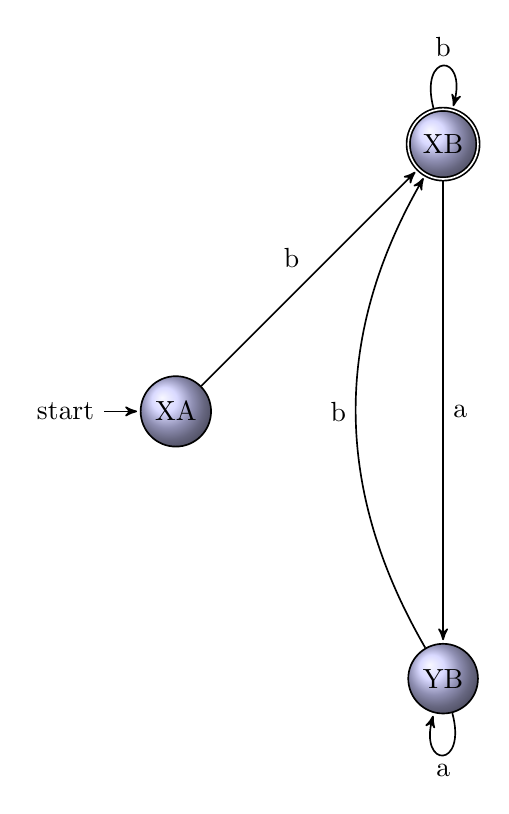
\begin{tikzpicture}[->,>=stealth',shorten >=1pt,auto,node distance=4.8cm, semithick]
\tikzstyle{every state}=[draw=black,text=black, ball color=blue!20]
\node[initial,state] (XA) {XA};
\node[state,accepting][above right of=XA](XB){XB};
\node[state][below right of=XA](YB){YB};
\path (XA)edge node{b}(XB)
         (XB)edge  [loop above]node{b}(XB)
               edge node{a}(YB)
         (YB)edge [loop below]node{a}(YB)
               edge [bend left]node{b}(XB);
\end{tikzpicture} 
\end{center}
\end{figure}
\clearpage

\begin{figure}
\begin{center}
\caption{Q02: $L_1$ = (a+b)b(a+b)*}
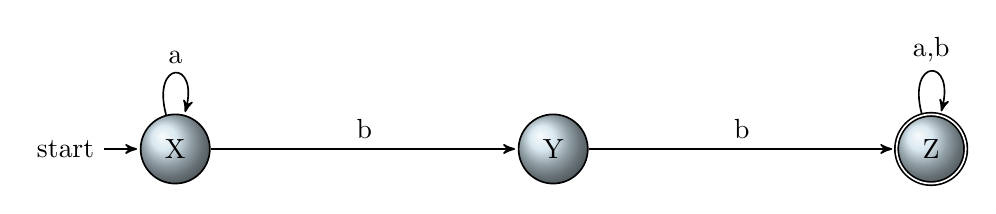
\begin{tikzpicture}[->,>=stealth',shorten >=1pt,auto,node distance=4.8cm, semithick]
\tikzstyle{every state}=[draw=black,text=black, ball color=green!40!blue!20!]
\node[initial,state] (X) {X};
\node[state] [right of=X](Y){Y};
\node[state,accepting][right of=Y](Z){Z};
\path (X)edge [loop above]node{a}(X)
              edge node{b}(Y)
              (Y)edge node{b}(Z)
          (Z)edge [loop above]node{a,b}(Z);   
\end{tikzpicture} 
\end{center}
\end{figure}

\begin{figure}
\begin{center}
\caption{Q02: $L_2$= b(a+b)*}
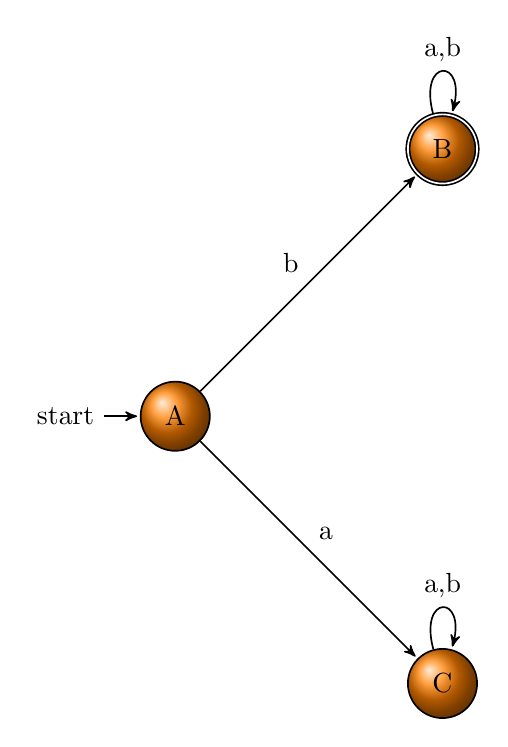
\begin{tikzpicture}[->,>=stealth',shorten >=1pt,auto,node distance=4.8cm, semithick]
\tikzstyle{every state}=[draw=black,text=black, ball color=orange]
\node[initial,state] (A) {A};
\node[state,accepting][above right of=A](B){B};
\node[state][below right of=A](C){C};
\path (A)edge node{b}(B)
         edge  node{a}(C)
      (B)edge  [loop above]node{a,b}(B)
      (C)edge [loop above]node{a,b}(C);
\end{tikzpicture} 
\end{center}
\end{figure}

\begin{figure}
\begin{center}
\caption{Q02: $L_1$$\bigcap$$L_2$}
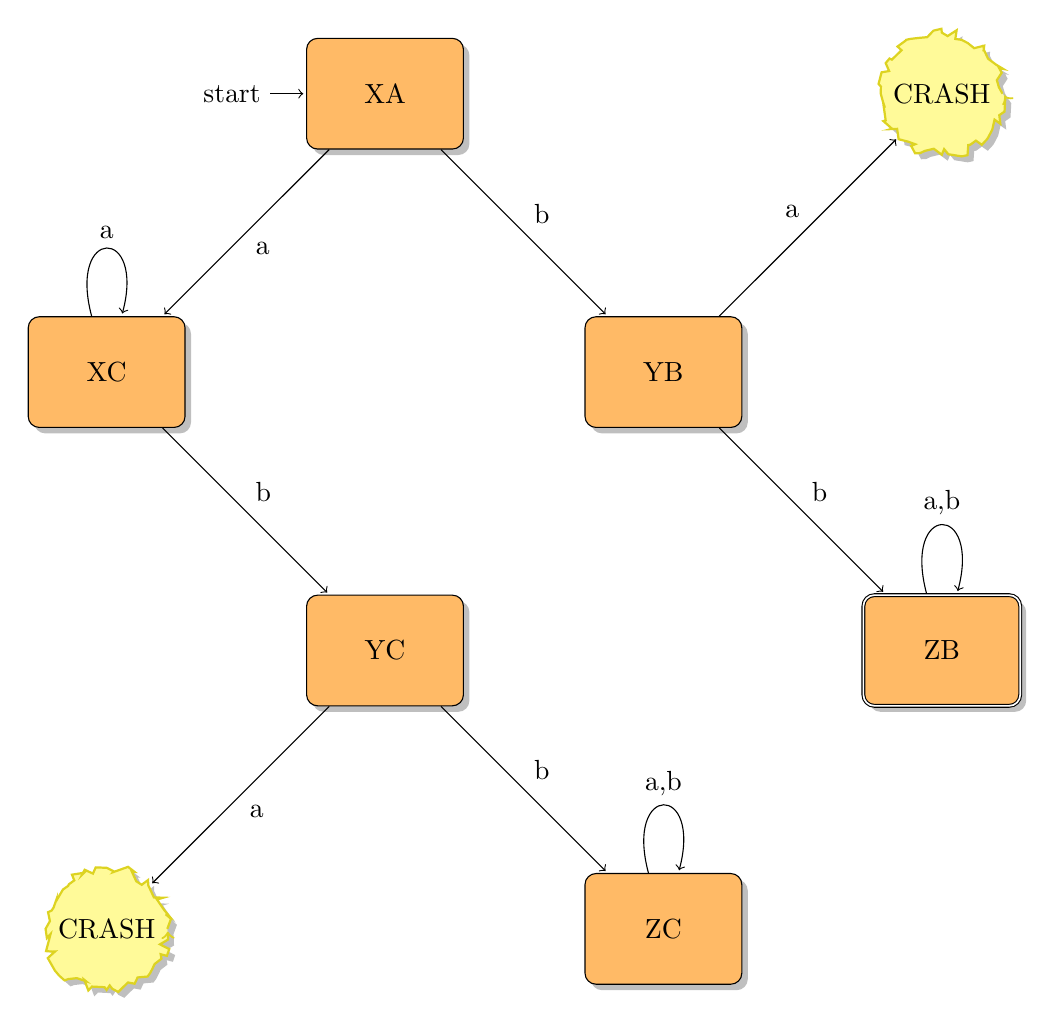
\begin{tikzpicture}[->,shorten >=1pt,node distance=5cm,auto]
\tikzstyle{every state} = [rectangle, draw, fill=red!45!yellow!60!, text width=5em, text centered, rounded corners, minimum height=4em, drop shadow]
\tikzstyle{noise}=[circle,
                                    thick,
                                    minimum size=1.2cm,
                                    draw=yellow!85!black,
                                    fill=yellow!40,
                                    decorate,
                                    drop shadow,
                                    decoration={random steps,
                                                            segment length=2pt,
                                                            amplitude=2pt}]
\node[initial,state] (XA){XA};
\node[state][below left of=XA](XC){XC};
\node[state][below right of=XC](YC){YC};
\node[state][below right of=YC](ZC){ZC};
\node[noise][below left of=YC](CRASH){CRASH};
\node[state][below right of=XA](YB){YB};
\node[noise][above right of=YB](CRASH2){CRASH};
\node[state, accepting][below right of=YB](ZB){ZB};
\path (XA)edge node{a}(XC)
                edge node{b}(YB)
          (XC)edge [loop above]node{a}(XC)
                edge node{b}(YC)
          (YC)edge node{a}(CRASH)
                edge node{b}(ZC)
          (ZC)edge [loop above] node{a,b}(ZC)
          (ZB)edge [loop above]node{a,b}(ZB)
          (YB)edge node{a}(CRASH2)
                edge node{b}(ZB);
\end{tikzpicture}
\end{center}
\end{figure}

\begin{figure}
\begin{center}
\caption{Q02: $L_3$ = bb(a+b)*}
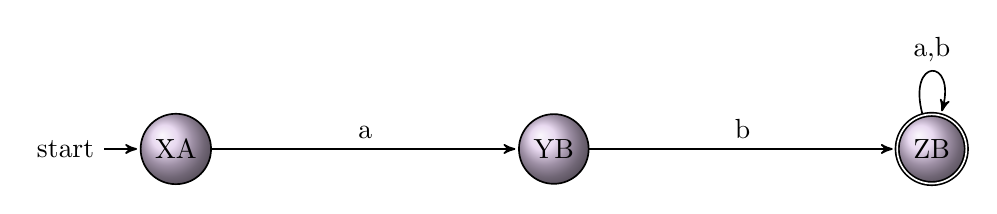
\begin{tikzpicture}[->,>=stealth',shorten >=1pt,auto,node distance=4.8cm, semithick]
\tikzstyle{every state}=[draw=black,text=black, ball color=red!40!blue!20!]
\node[initial,state] (XA) {XA};
\node[state] [right of=XA](YB){YB};
\node[state,accepting][right of=YB](ZB){ZB};
\path (XA)edge node{a}(YB)
          (YB)edge node{b}(ZB)
          (ZB)edge [loop above]node{a,b}(ZB); 
\end{tikzpicture} 
\end{center}
\end{figure}

\begin{figure}
\begin{center}
\caption{Q03: $L_1$ = (b+ab)*(a+$\Lambda$)}
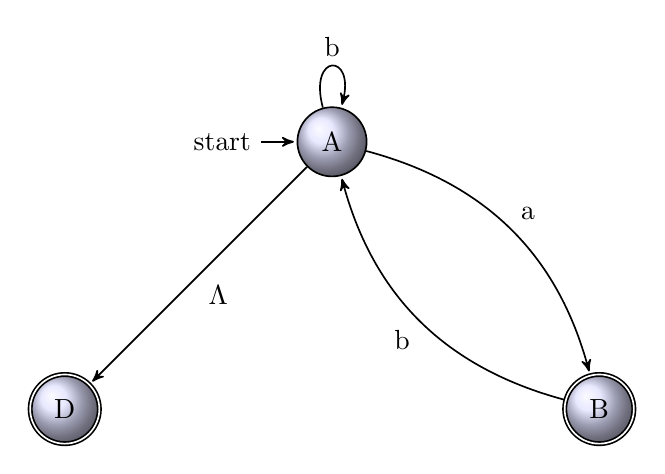
\begin{tikzpicture}[->,>=stealth',shorten >=1pt,auto,node distance=4.8cm, semithick]
\tikzstyle{every state}=[draw=black,text=black, ball color=white!40!blue!20!]
\node[initial,state] (A) {A};
\node[state,accepting] [below right of=A](B){B};
\node[state,accepting][below left of=A](D){D};
\path (A)edge [bend left]node{a}(B)
              edge [loop above]node{b}(A)
              edge node{$\Lambda$}(D)
          (B)edge [bend left]node{b}(A);
            
             
\end{tikzpicture} 
\end{center}
\end{figure}

\begin{figure}
\begin{center}
\caption{Q03: $L_2$ = (a+b)*aa(a+b)*}
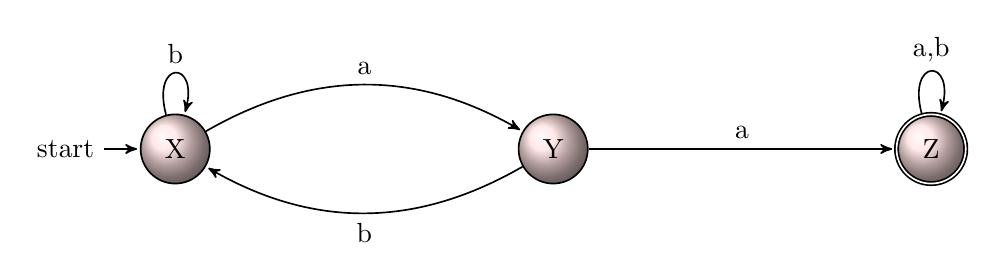
\begin{tikzpicture}[->,>=stealth',shorten >=1pt,auto,node distance=4.8cm, semithick]
\tikzstyle{every state}=[draw=black,text=black, ball color=white!40!red!20!]
\node[initial,state] (X) {X};
\node[state][right of=X](Y){Y};
\node[state,accepting][right of=Y](Z){Z};
\path (X)edge [bend left]node{a}(Y)
              edge[loop above]node{b}(X)
         (Y)edge node{a}(Z)
              edge [bend left]node{b}(X)
         (Z)edge [loop above]node{a,b}(Z);
\end{tikzpicture} 
\end{center}
\end{figure}

\begin{figure}
\begin{center}
\caption{Q02: $L_1$$\bigcap$$L_2$}
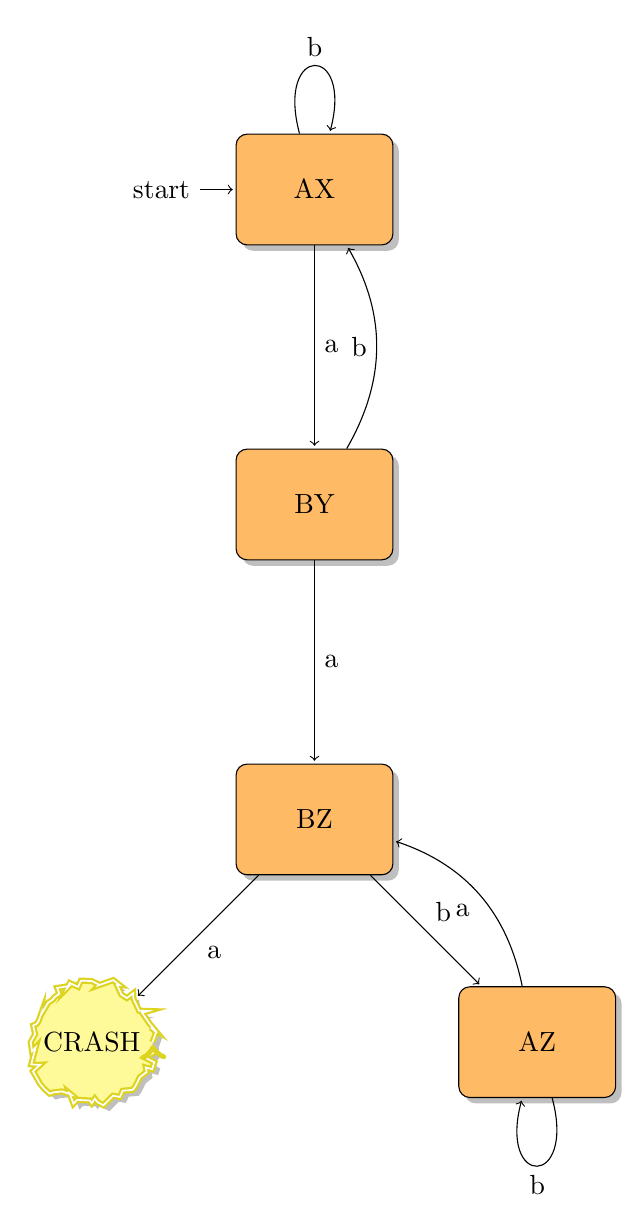
\begin{tikzpicture}[->,shorten >=1pt,node distance=4cm,auto]
\tikzstyle{every state} = [rectangle, draw, fill=red!45!yellow!60!, text width=5em, text centered, rounded corners, minimum height=4em, drop shadow]
\tikzstyle{noise}=[circle,
                                    thick,
                                    minimum size=1.2cm,
                                    draw=yellow!85!black,
                                    fill=yellow!40,
                                    decorate,
                                    drop shadow,
                                    decoration={random steps,
                                                            segment length=2pt,
                                                            amplitude=2pt}]
\node[initial,state] (AX){AX};
\node[state][below of=AX](BY){BY};
\node[state][below of=BY](BZ){BZ};
\node[noise,accepting][below left of=BZ](CRASH){CRASH};
\node[state][below right of=BZ](AZ){AZ};
\path (AX)edge node{a}(BY)
                edge [loop above]node{b}(AX)
          (BY)edge node{a}(BZ)
                edge [bend right]node{b}(AX)
          (BZ)edge node{b}(AZ)
                edge node{a}(CRASH)
          (AZ)edge [bend right]node{a}(BZ)
                edge [loop below]node{b}(AZ);
         
\end{tikzpicture}
\end{center}
\end{figure}
\begin{figure}
\begin{center}
\caption{Q03: $L_3$ = (a+b)*aaba}
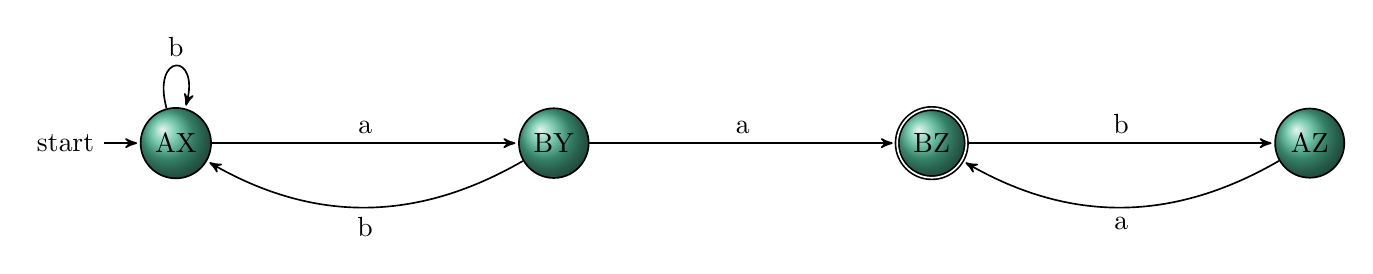
\begin{tikzpicture}[->,>=stealth',shorten >=1pt,auto,node distance=4.8cm, semithick]
\tikzstyle{every state}=[draw=black,text=black, ball color=blue!40!green!70!]
\node[initial,state] (AX) {AX};
\node[state][right of=AX](BY){BY};
\node[state,accepting][right of=BY](BZ){BZ};
\node[state][right of=BZ](AZ){AZ};
\path (AX)edge [loop above]node{b}(AX)
                edge node{a}(BY)
          (BY)edge [bend left]node{b}(AX)
                edge node{a}(BZ)
          (BZ)edge node{b}(AZ)
          (AZ)edge [bend left]node{a}(BZ);   
\end{tikzpicture} 
\end{center}
\end{figure}

\end{document}